% ======================= CHAPTER 4: EXPERIMENTS AND RESULTS ==========================
\chapter{Experiments and Results}

All experiments were run on the single 4~GB GPU described in Section~3.3, with the random seed fixed at 42. Results are reported on the held-out test set of twenty videos (IDs 61--80), which no model saw during training or model selection.

\section{Comparison of the Three Models}

\subsection{Overall Results}

Table~\ref{tab:model_comparison} reports accuracy and macro-F1 for the three models, before and after median smoothing.

\begin{table}[H]
\centering
\caption{Test-set results for the three models. Best values in \textbf{bold}.}
\label{tab:model_comparison}
\begin{tabular}{lcccc}
\toprule
\textbf{Model} & \textbf{Raw Acc.} & \textbf{Raw Macro-F1} & \textbf{Smoothed Acc.} & \textbf{Smoothed Macro-F1} \\
\midrule
M1 --- ResNet-50 + BiLSTM      & 0.832 & 0.775 & 0.837 & 0.781 \\
M2 --- EfficientNet-B3 + TCN   & 0.818 & 0.739 & 0.824 & 0.748 \\
\textbf{M3 --- Swin-Tiny + Transformer} & \textbf{0.857} & \textbf{0.807} & \textbf{0.862} & \textbf{0.815} \\
\bottomrule
\end{tabular}
\end{table}

The Swin-Transformer M3 is best on every metric, with a smoothed macro-F1 of \textbf{0.815}---3.4 points above the ResNet-LSTM and 6.7 points above the EfficientNet-TCN. Its accuracy of 0.862 is in the same range as Trans-SVNet~\cite{gao2021transsvnet} on this dataset, even though it was trained on a single 4~GB laptop GPU. Figure~\ref{fig:arch_compare} plots each model's score against its number of parameters: M3 wins without being the largest model, and M1 has more parameters yet scores lower, so model size is not what limits the result here.

\begin{figure}[H]
\centering
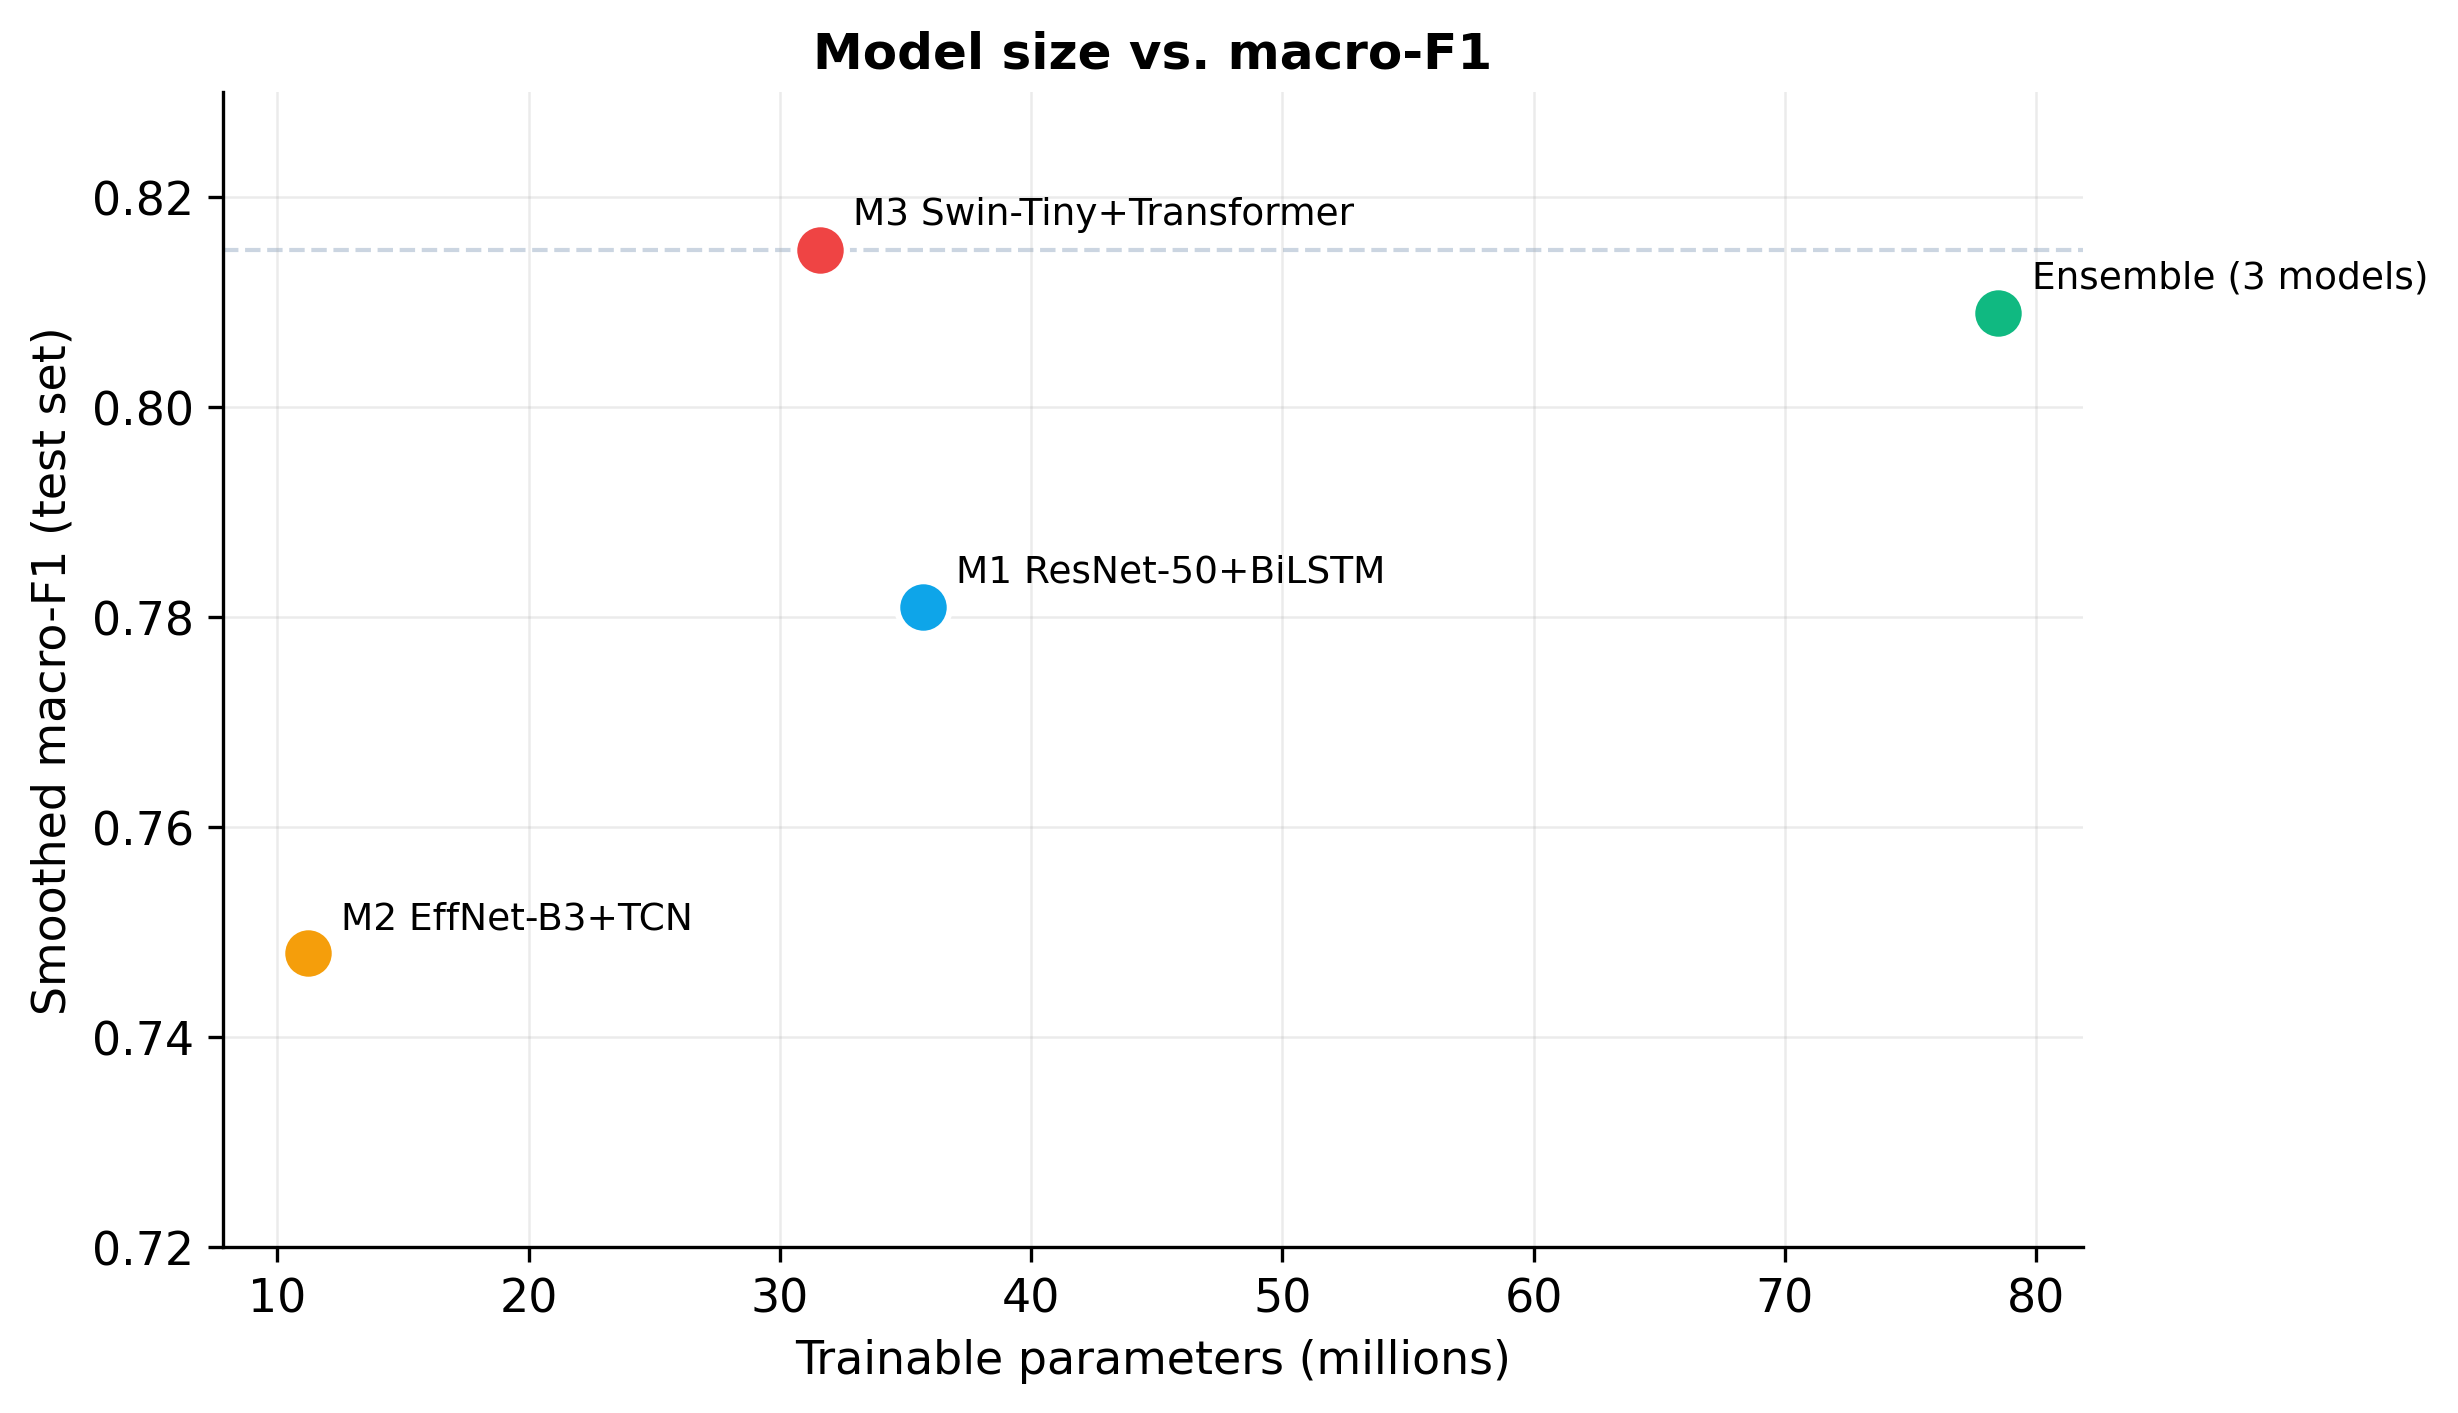
\includegraphics[width=\figwidth]{figures/arch_compare.png}
\caption{Model size versus macro-F1. The Swin-Transformer (M3) scores highest without being the largest; the EfficientNet-TCN (M2) is the smallest and the weakest, partly because its Stage-3 fine-tuning was cut short by limited memory.}
\label{fig:arch_compare}
\end{figure}

\subsection{Training Dynamics}

Figure~\ref{fig:training_history} shows the loss and accuracy curves for the three models over the three stages. M1 and M3 train smoothly, and their validation accuracy jumps once the backbone is unfrozen in Stage 3. M2's curve is shorter: with the EfficientNet-B3 backbone unfrozen, memory use reached about 97\% of the 4~GB limit and only part of Stage 3 finished, so M2's numbers are a lower bound on what it could reach with more memory.

\begin{figure}[H]
\centering
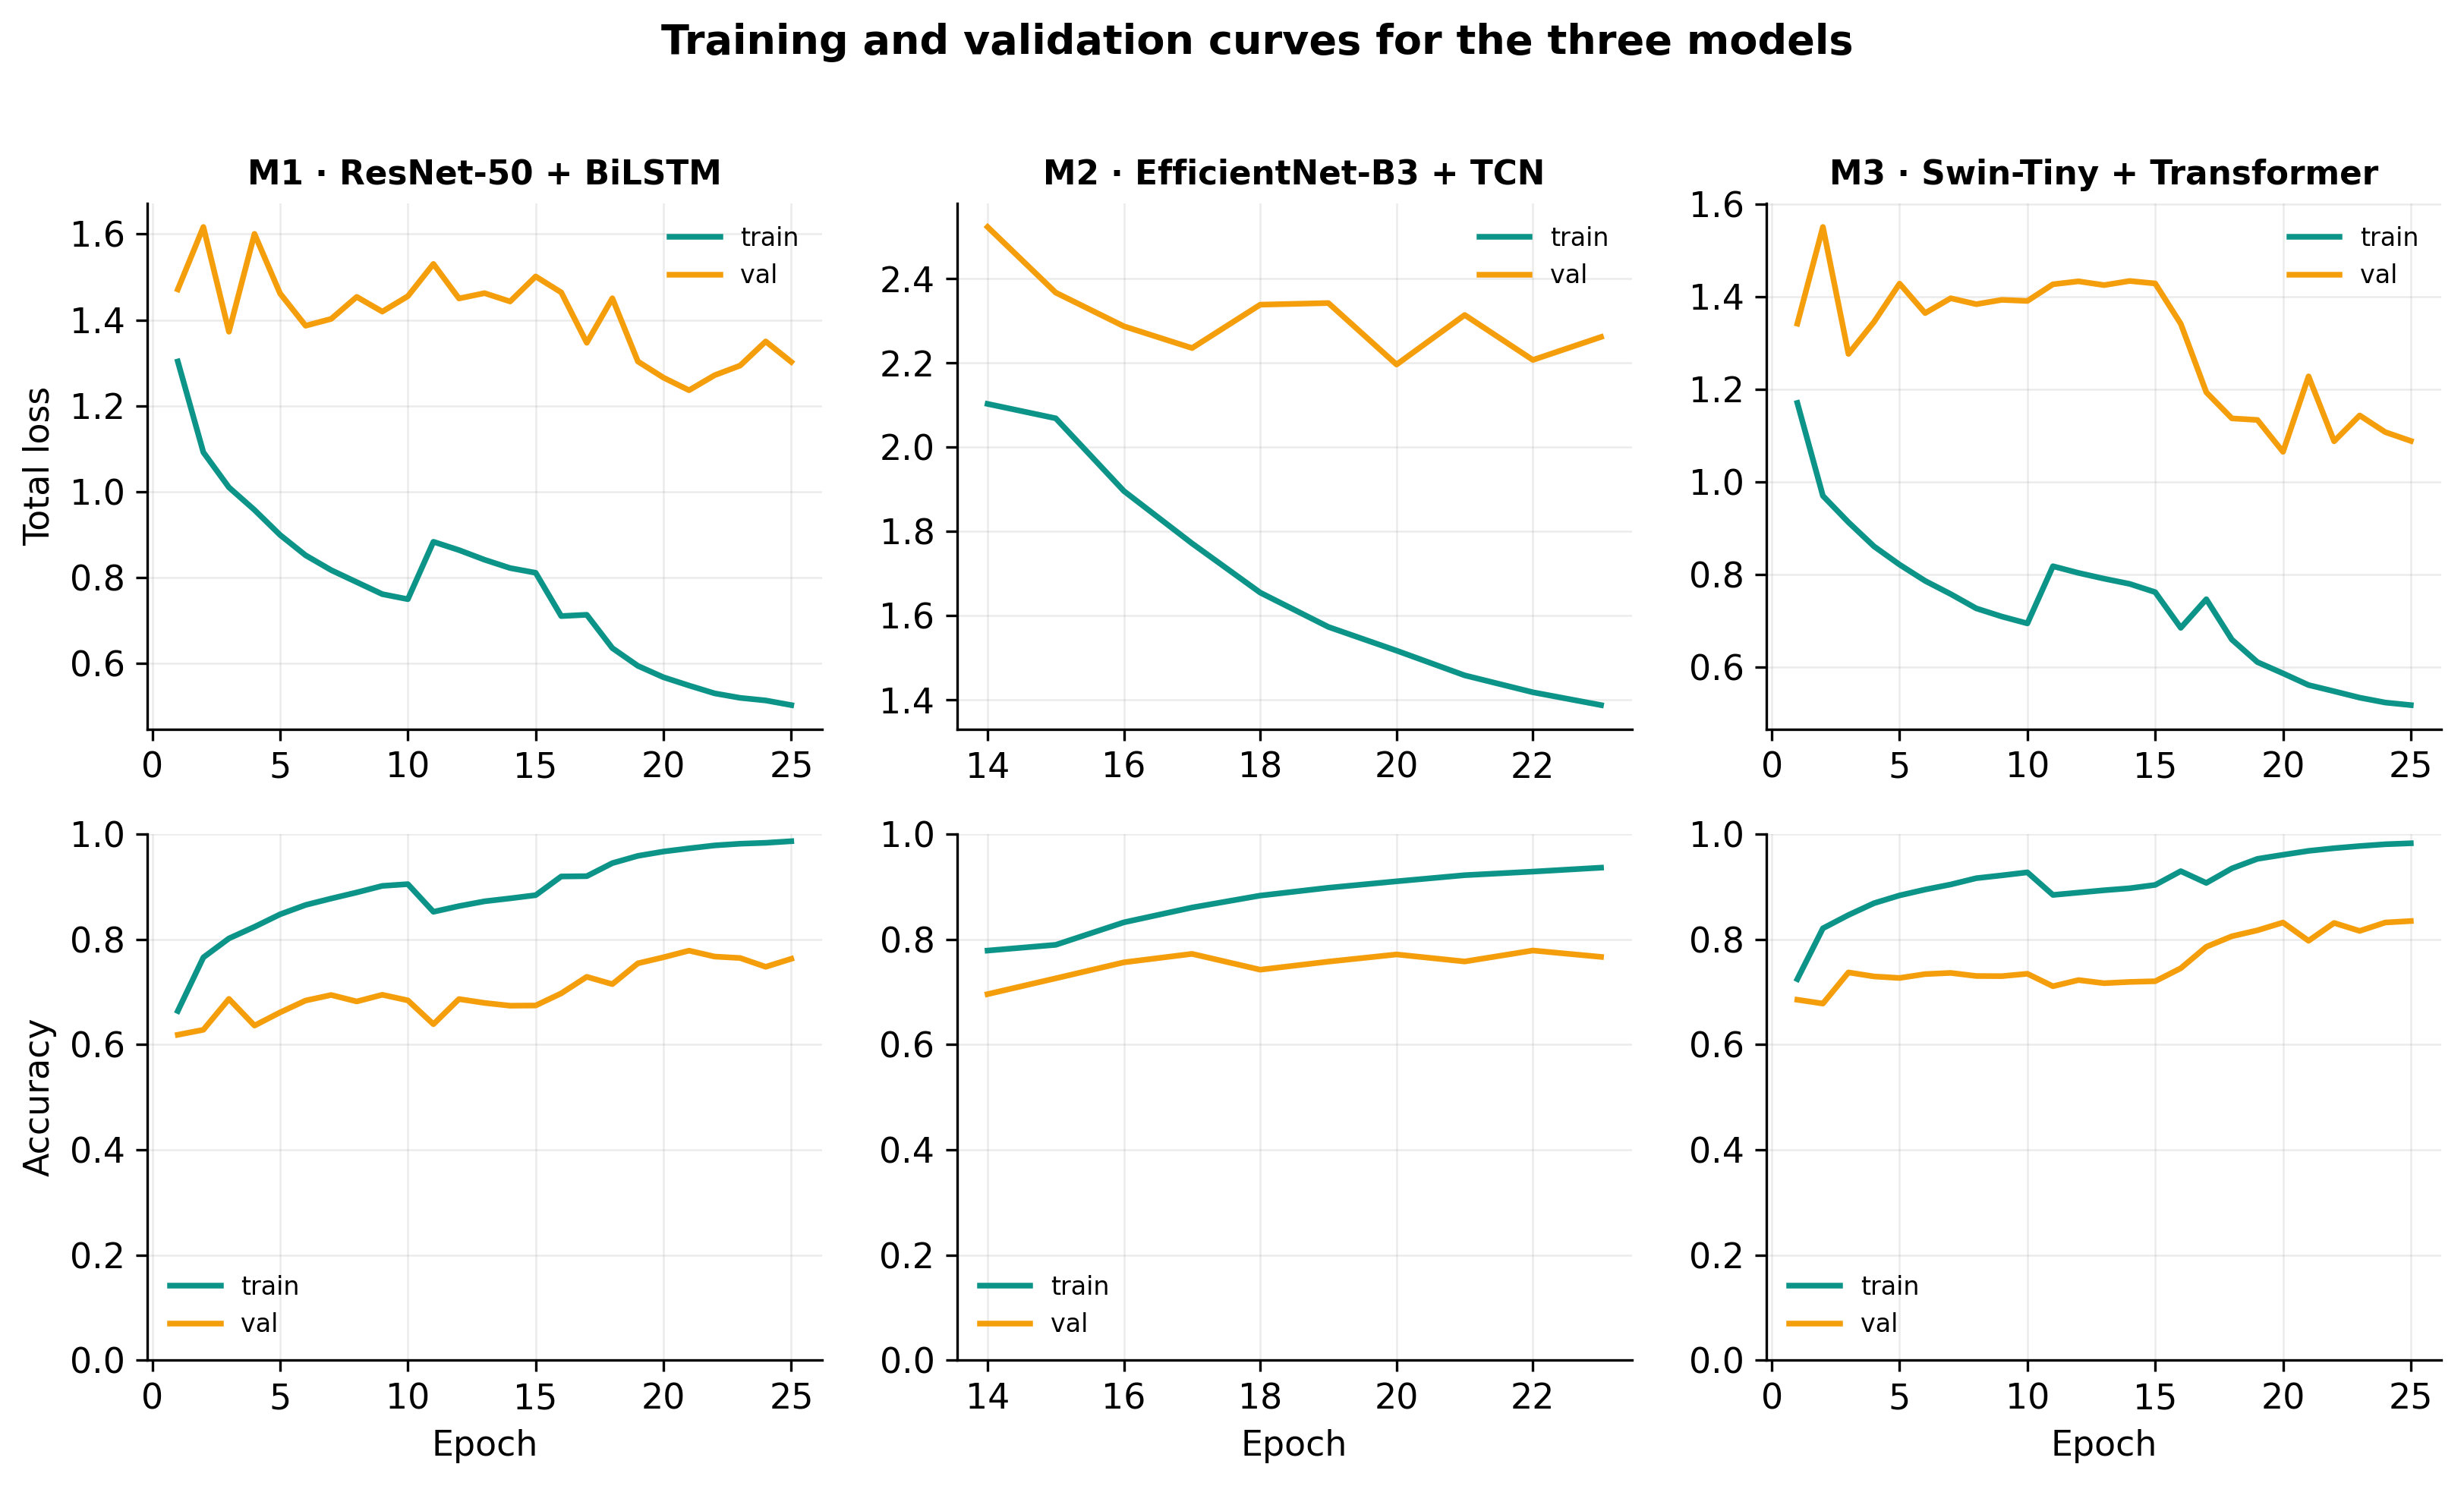
\includegraphics[width=\textwidth]{figures/train_history.png}
\caption{Training and validation loss and accuracy over epochs for the three models. M3 shows the clearest jump in Stage 3; M2's run is cut short by limited memory during backbone fine-tuning.}
\label{fig:training_history}
\end{figure}

\subsection{Per-Phase Analysis}

Table~\ref{tab:per_class_m3} details per-class precision, recall, and F1 for M3 on the raw test predictions.

\begin{table}[H]
\centering
\caption{Per-phase precision, recall, and F1 for M3 (raw predictions, test set). The weakest phase is in \textbf{bold}.}
\label{tab:per_class_m3}
\begin{tabular}{lccc}
\toprule
\textbf{Phase} & \textbf{Precision} & \textbf{Recall} & \textbf{F1} \\
\midrule
Preparation               & 0.830 & 0.803 & 0.816 \\
Calot triangle dissection & 0.880 & 0.895 & 0.887 \\
Clipping and cutting      & 0.815 & 0.796 & 0.806 \\
Gallbladder dissection    & 0.868 & 0.885 & 0.877 \\
Gallbladder packaging     & 0.881 & 0.759 & 0.816 \\
Cleaning and coagulation  & 0.741 & 0.663 & \textbf{0.700} \\
Gallbladder retraction    & 0.727 & 0.764 & 0.745 \\
\bottomrule
\end{tabular}
\end{table}

The two common phases have the highest F1, as expected. The weakest is Cleaning and coagulation (recall 0.663): the model often mistakes cleaning for the surrounding dissection phase, which also shows up in the confusion matrix (Figure~\ref{fig:confusion_m3}). Importantly, all seven phases are above F1 $=0.70$, so the class-weighted loss does prevent the model from collapsing onto the common phases.

\begin{figure}[H]
\centering
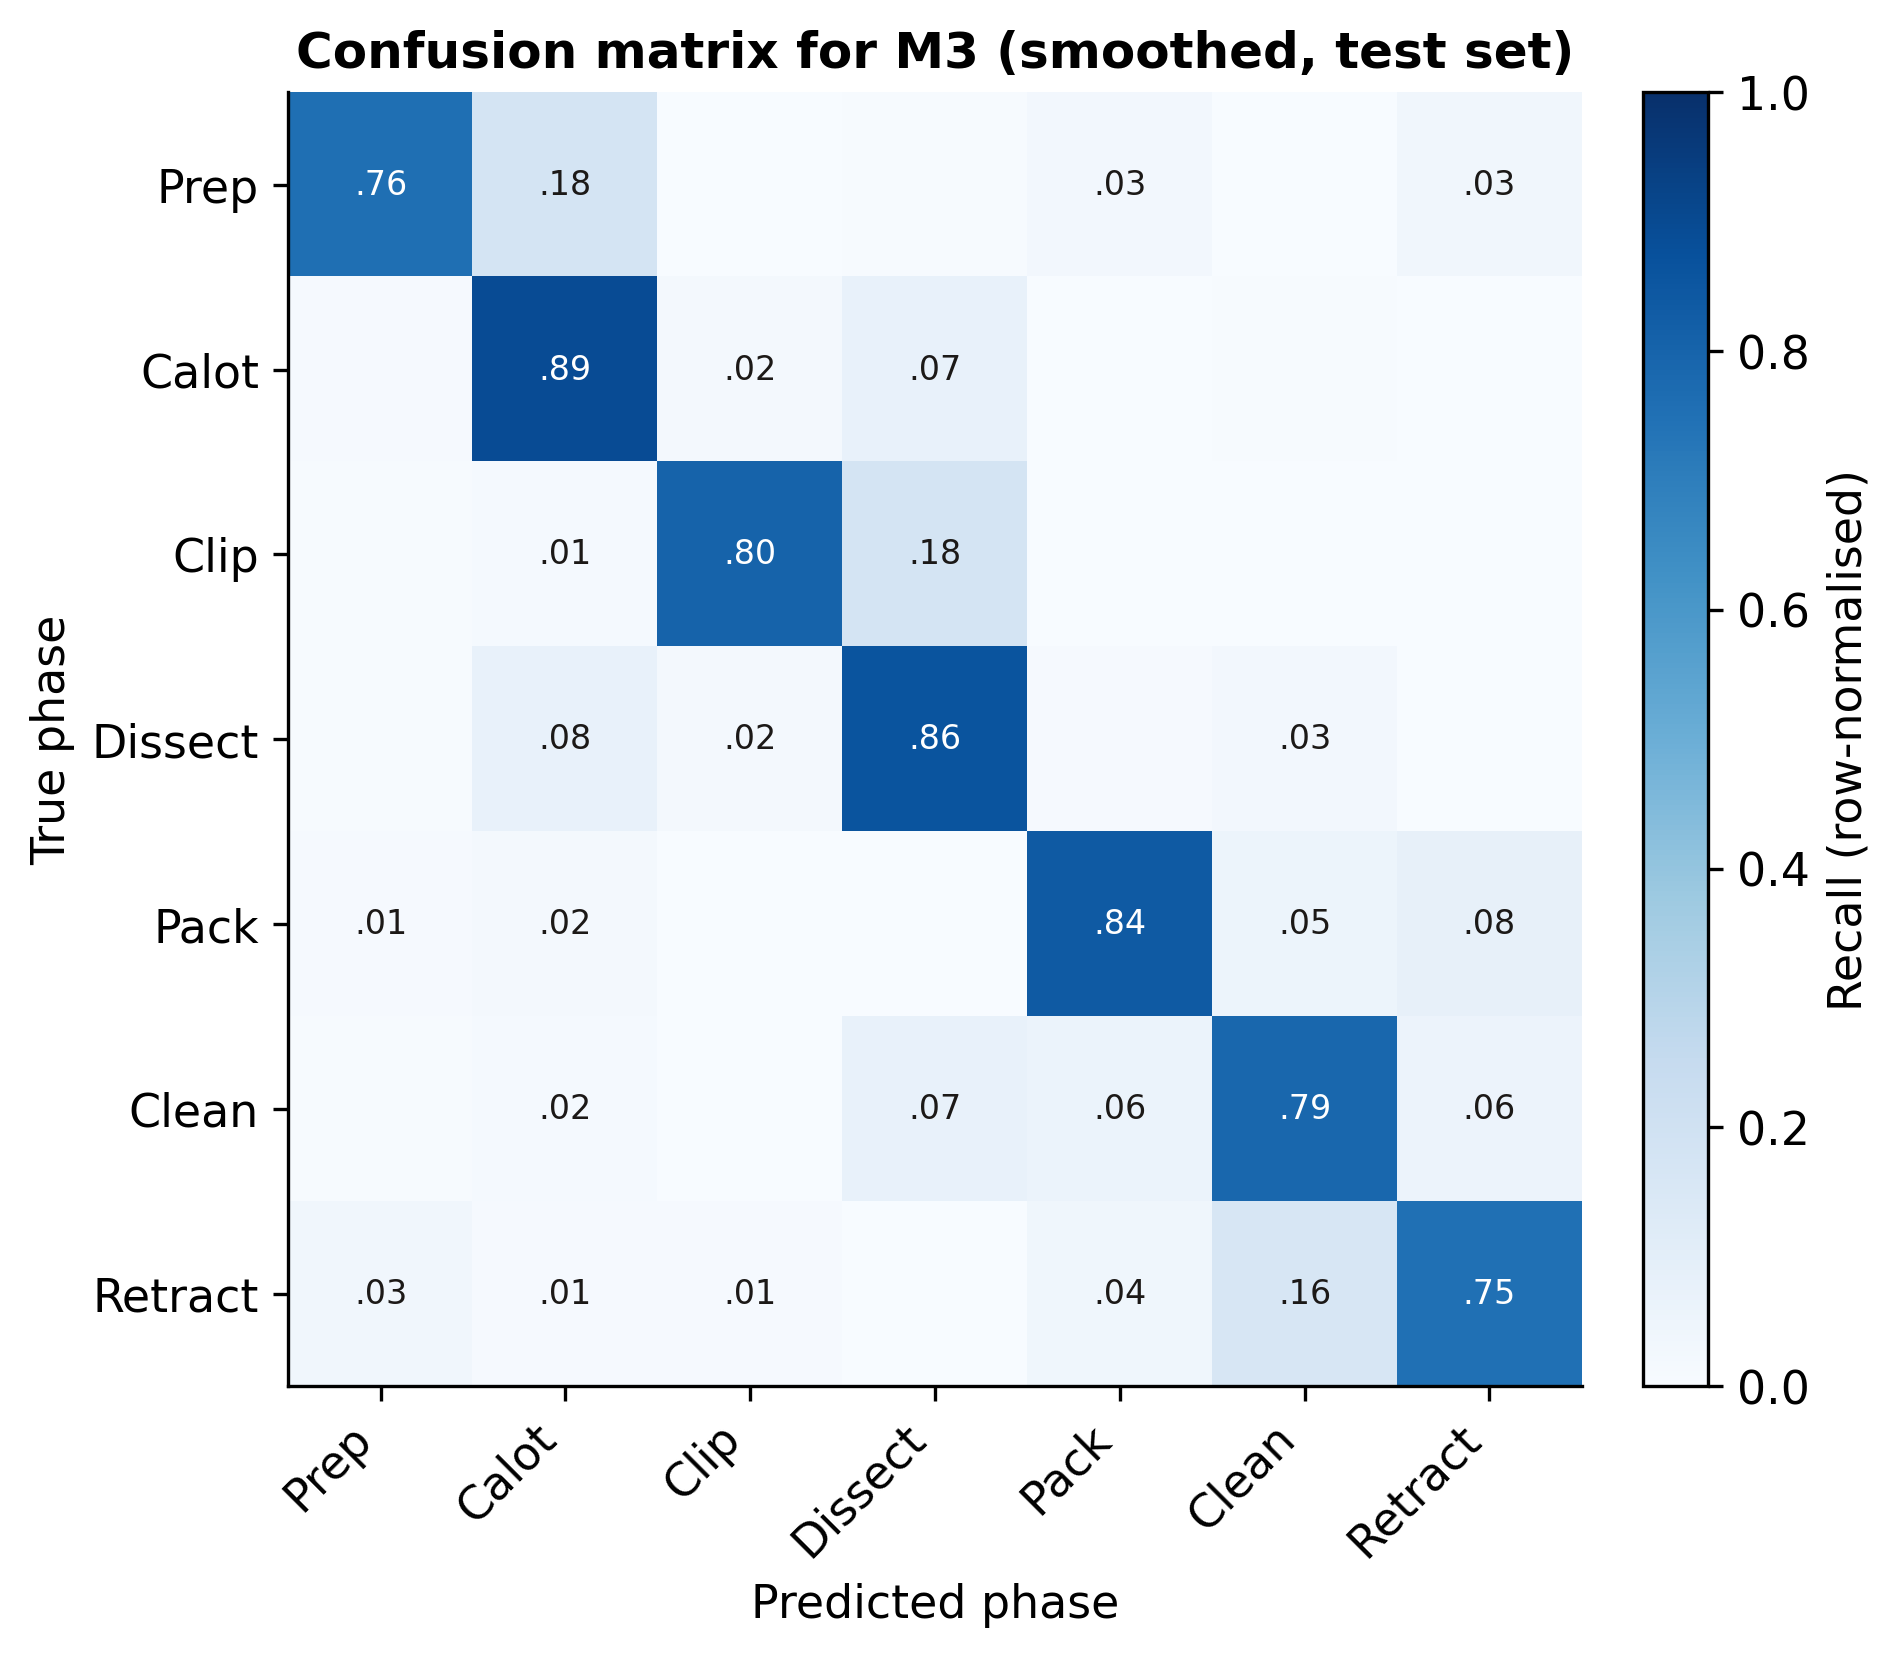
\includegraphics[width=\figwidth]{figures/confusion_m3.png}
\caption{Confusion matrix (each row adds to 1) for M3 on the smoothed test predictions. The main mistakes are Cleaning and Clipping predicted as Dissection---neighbouring phases that look similar---and no phase collapses onto the common ones.}
\label{fig:confusion_m3}
\end{figure}

\section{Ablation Study}
\label{sec:ablation}

Table~\ref{tab:ablation} reports the four ablations against the M1 baseline, all trained with the same optimiser and three-stage schedule.

\begin{table}[H]
\centering
\caption{Ablation study (test-set smoothed macro-F1, change relative to M1).}
\label{tab:ablation}
\begin{tabular}{llcc}
\toprule
\textbf{ID} & \textbf{Modification} & \textbf{Smoothed Macro-F1} & \textbf{$\Delta$F1 vs M1}\\
\midrule
\textbf{M1 baseline} & full configuration & \textbf{0.781} & --- \\
\midrule
A1 & remove tool detection (single-task) & 0.765 & $-1.6\%$ \\
A2 & remove class weighting              & 0.761 & $-2.0\%$ \\
A3 & sequence length 16 instead of 8     & 0.787 & $+0.6\%$ \\
A4 & disable median smoothing            & 0.775 & $-0.6\%$ \\
\bottomrule
\end{tabular}
\end{table}

Three points stand out. First, removing the tool task (A1) costs 1.6 points of macro-F1, confirming that the extra task helps, as EndoNet first noted~\cite{twinanda2017endonet}. Second, removing class weighting (A2) costs 2.0 points, but the loss is uneven: the two rarest phases---Gallbladder retraction and packaging---drop 5.1 and 2.8 points of per-phase F1, while the common Calot phase actually gains 0.7. This is exactly the problem class weighting is meant to fix. Third, A4 shows what the median filter does: it barely changes macro-F1 ($+0.6\%$) but improves the edit score by about 35\%, so its main job is cleaning up the phase sequence, not improving per-frame accuracy. Doubling the sequence length (A3) gives only $+0.6\%$, which means the eight-second window already covers most of the useful context.

Together, class weighting and the tool task are worth almost four points of macro-F1---about the same as the 3.4-point gap between the best and worst architecture. This is the main evidence that, on Cholec80, the training recipe matters as much as the backbone.

\section{Ensemble Results}

Table~\ref{tab:ensemble} compares the three ways of combining the models.

\begin{table}[H]
\centering
\caption{Combining the three models (smoothed, test set). Best values in \textbf{bold}.}
\label{tab:ensemble}
\begin{tabular}{lcc}
\toprule
\textbf{Strategy} & \textbf{Accuracy} & \textbf{Macro-F1} \\
\midrule
M3 alone (best single model)              & 0.856 & 0.799 \\
Ensemble --- simple softmax average       & 0.863 & 0.808 \\
\textbf{Ensemble --- val-F1-weighted average} & \textbf{0.864} & \textbf{0.809} \\
Ensemble --- majority voting              & 0.857 & 0.799 \\
\bottomrule
\end{tabular}
\end{table}

The F1-weighted average beats the best single model by 1.0 point of macro-F1, with M3 getting the largest weight (0.355), then M1 (0.327) and M2 (0.318). The weights are almost equal, which suggests the three models are each capable but make similar mistakes---they tend to be wrong on the same hard frames (usually near phase changes) rather than on different ones. This is why the next section turns to decoding and calibration: if the remaining errors are concentrated and structured, a better decoder may help more than adding more models.

\section{Real-Time Decoding and Calibration}
\label{sec:calibration}

This section compares the real-time decoder of Section~\ref{sec:decoding} with the baselines, using the same per-frame scores for every method so that any difference comes only from the decoding step.

\subsection{Calibration}

Table~\ref{tab:calibration} reports validation ECE and NLL before and after temperature scaling. M1, the most over-confident model, gains the most---its ECE drops by 66\%. For all three models the best temperature is above 1.0, the sign of over-confidence. Figure~\ref{fig:reliability} shows the reliability diagrams: the raw accuracy sits below the diagonal in the high-confidence bins, and temperature scaling pulls the curve back toward the diagonal.

\begin{table}[H]
\centering
\caption{Validation calibration before and after temperature scaling. Best ECE in \textbf{bold}.}
\label{tab:calibration}
\begin{tabular}{lccccc}
\toprule
\textbf{Model} & \textbf{$T^\star$} & \textbf{ECE raw} & \textbf{ECE cal} & \textbf{NLL raw} & \textbf{NLL cal} \\
\midrule
M1 --- ResNet-LSTM      & 1.30 & 0.109 & \textbf{0.037} & 0.897 & 0.855 \\
M2 --- EffNet-TCN       & 1.10 & 0.059 & 0.074 & 0.824 & 0.817 \\
M3 --- Swin-Transformer & 1.20 & 0.074 & 0.070 & 0.688 & 0.667 \\
\bottomrule
\end{tabular}
\end{table}

\begin{figure}[H]
\centering
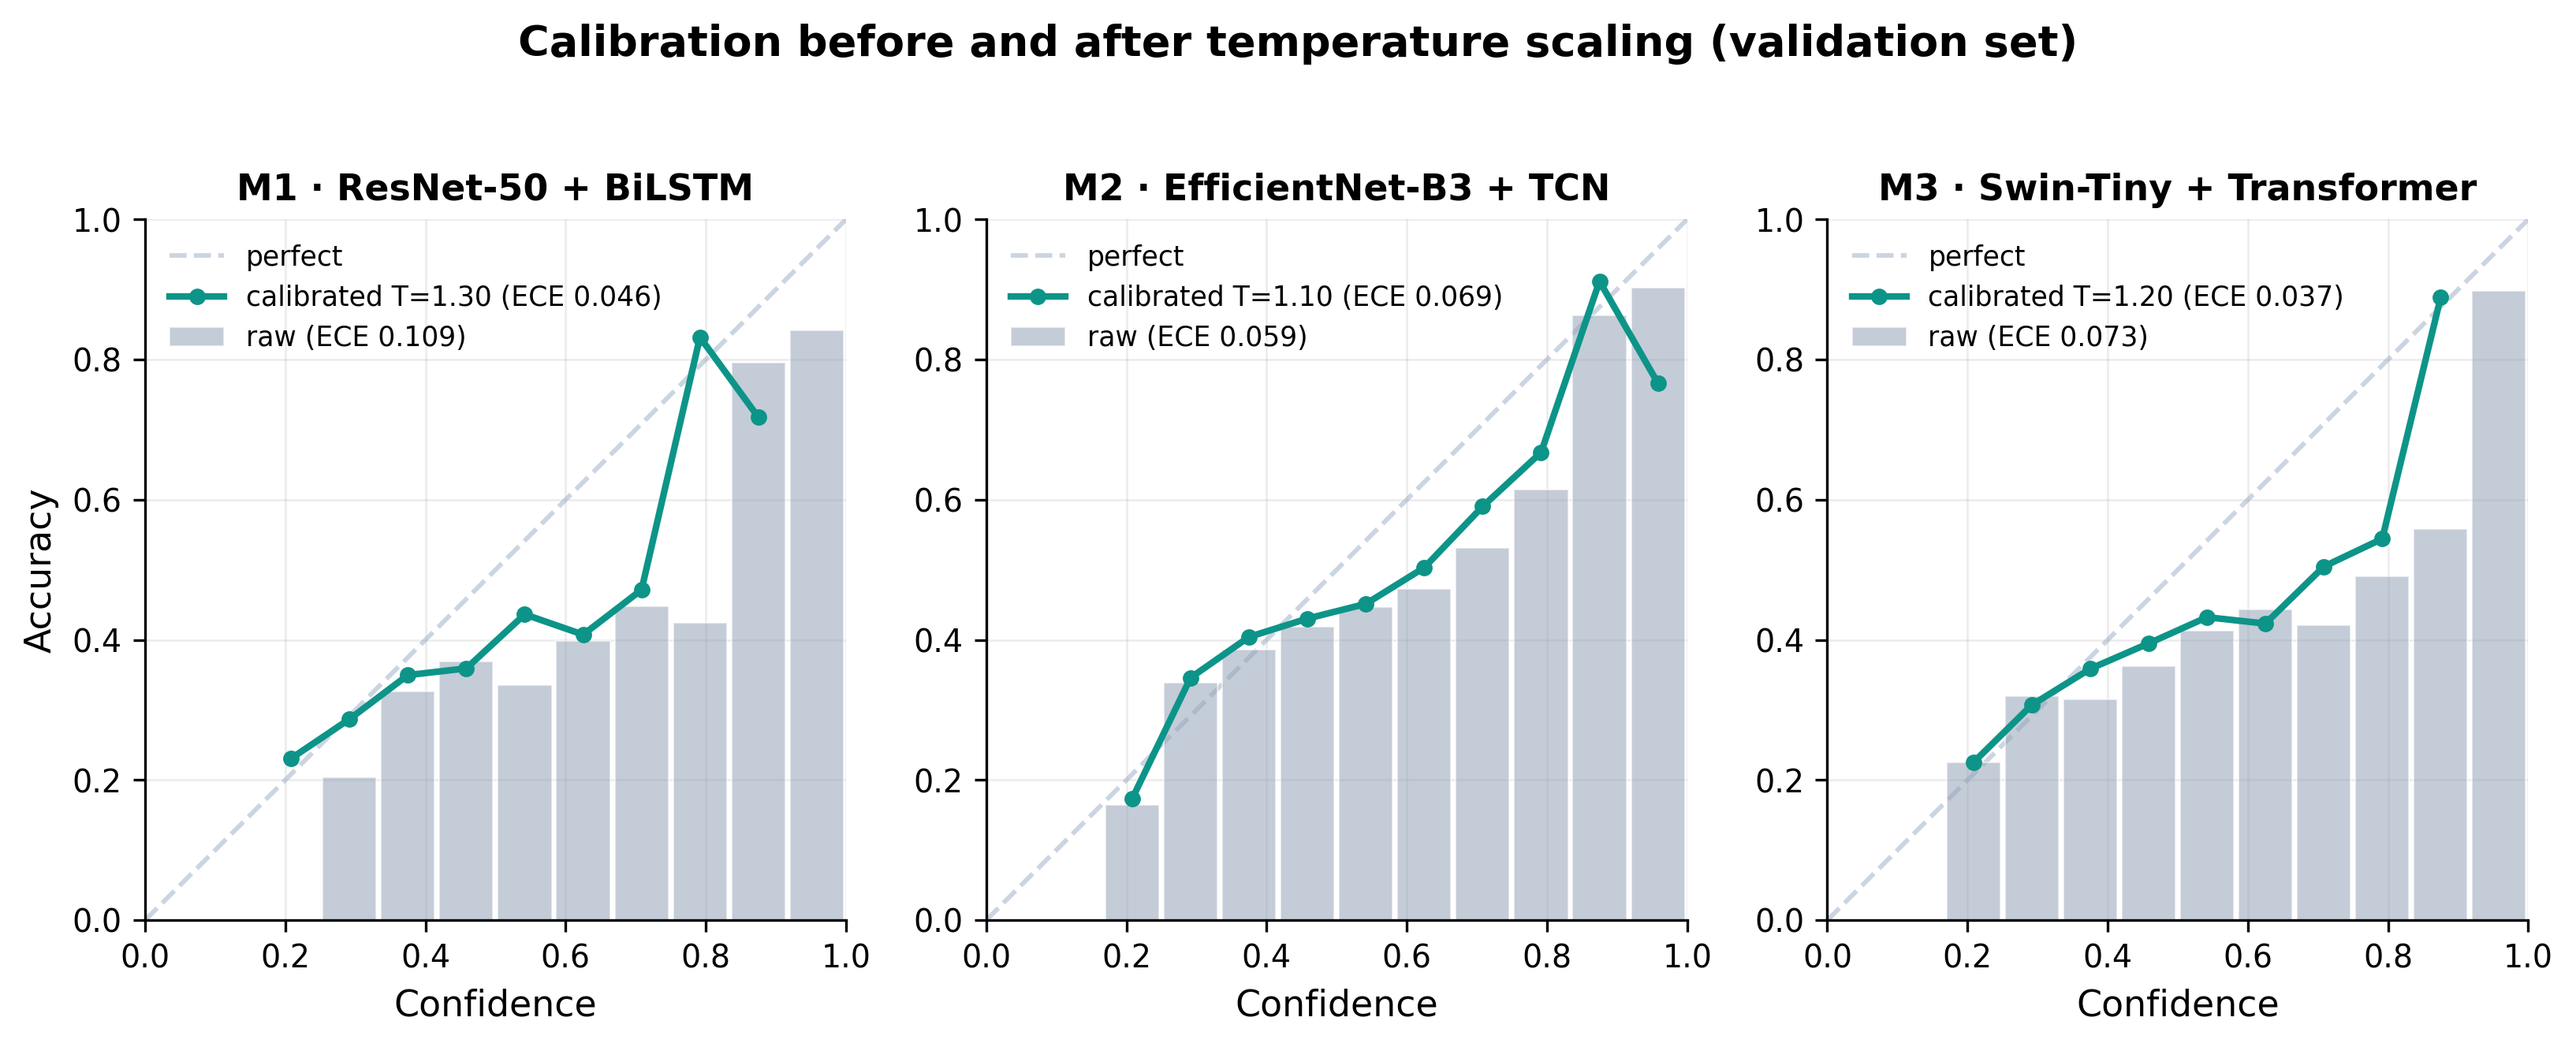
\includegraphics[width=\textwidth]{figures/reliability.png}
\caption{Reliability diagrams on the validation set. Grey bars are the raw accuracy in each confidence bin; the teal curve is after temperature scaling; the dashed diagonal is perfect calibration. M1 moves the most toward the diagonal.}
\label{fig:reliability}
\end{figure}

\subsection{Decoder Benchmark}

Table~\ref{tab:decoder} reports test accuracy and macro-F1 for each decoder on each model. The proposed decoder (calibrated scores plus the transition table) is the best real-time decoder on all three models; the offline decoder is shown only as an upper bound. Figure~\ref{fig:benchmark} shows the same comparison.

\begin{table}[H]
\centering
\caption{Decoder comparison (test set, accuracy / macro-F1). The offline decoder $\dagger$ uses future frames and is only an upper bound. Best \emph{real-time} values in \textbf{bold}.}
\label{tab:decoder}
\begin{tabular}{lccc}
\toprule
\textbf{Decoder} & \textbf{M1 Acc / F1} & \textbf{M2 Acc / F1} & \textbf{M3 Acc / F1} \\
\midrule
Raw predictions          & 82.4 / 0.763 & 81.2 / 0.738 & 85.3 / 0.794 \\
Median-15 filter         & 82.7 / 0.768 & 81.7 / 0.746 & 85.5 / 0.800 \\
Fixed-order + cal        & 82.5 / 0.777 & 82.4 / 0.767 & 86.0 / 0.802 \\
\textbf{Proposed decoder} & \textbf{83.0 / 0.771} & \textbf{82.9 / 0.764} & \textbf{86.0 / 0.806} \\
\midrule
Offline (full video) $\dagger$ & 91.8 / 0.859 & 91.8 / 0.849 & 90.1 / 0.832 \\
\bottomrule
\end{tabular}
\end{table}

\begin{figure}[H]
\centering
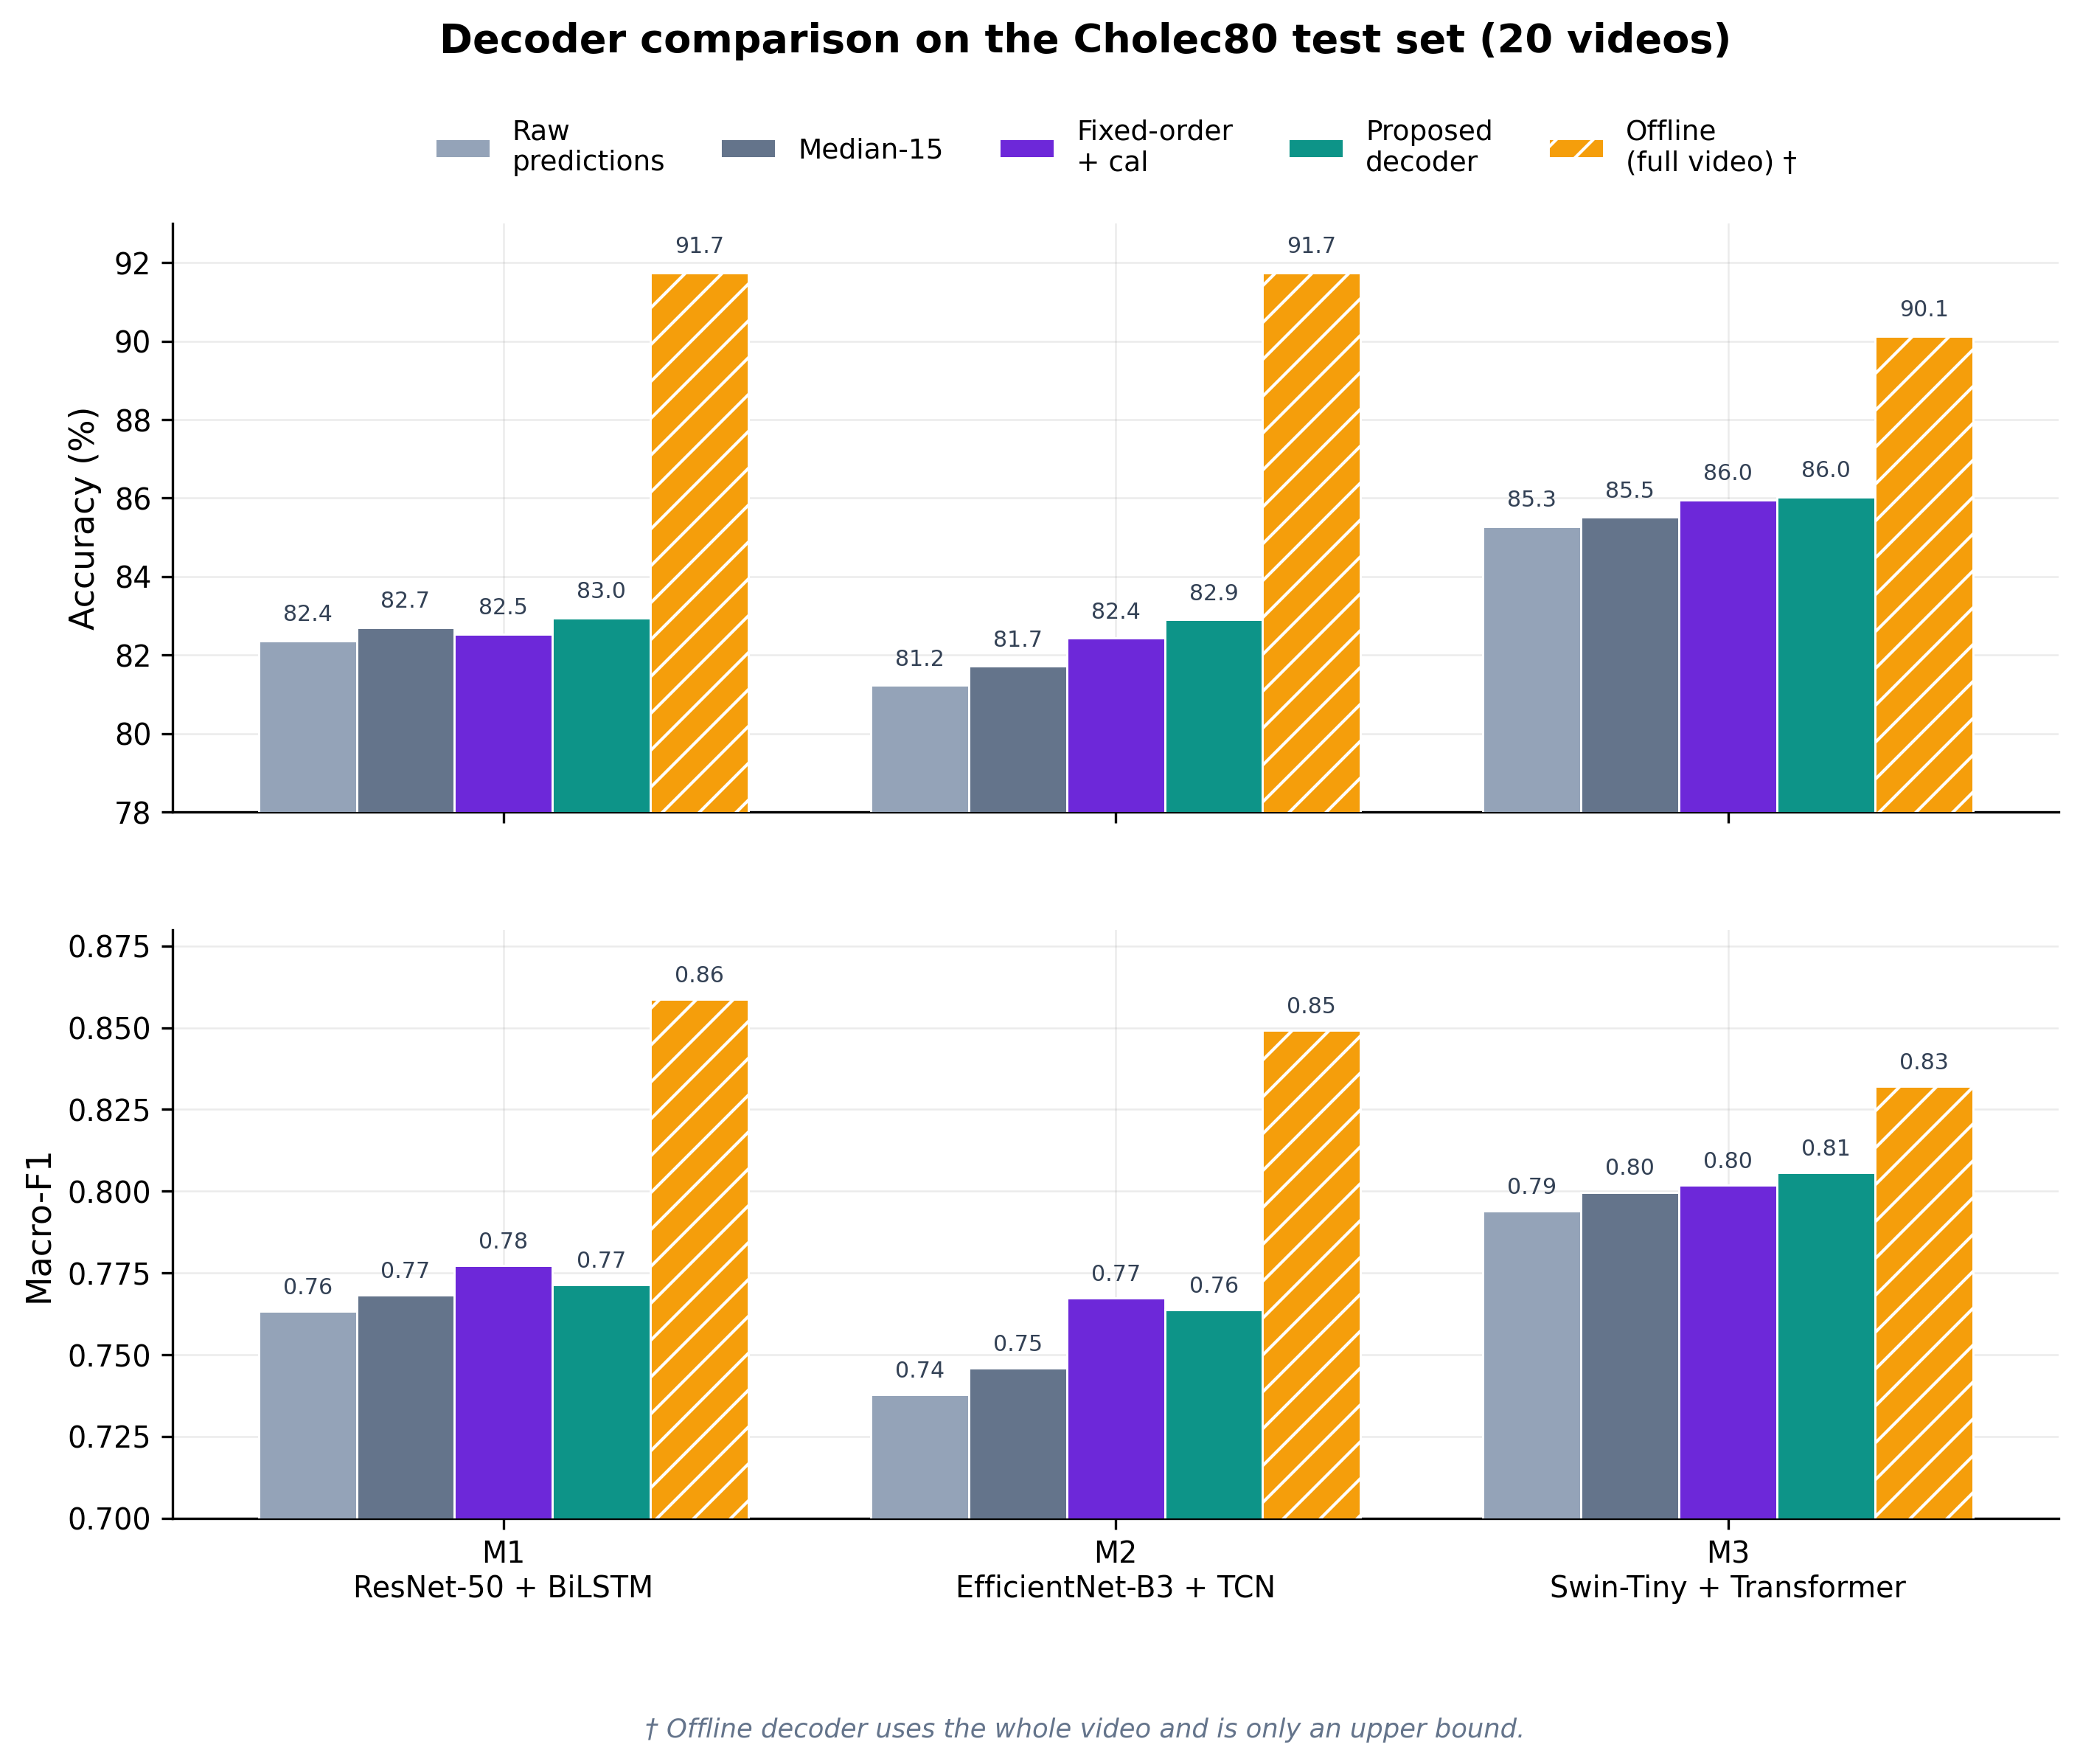
\includegraphics[width=\textwidth]{figures/benchmark.png}
\caption{Decoder comparison on the test set: accuracy and macro-F1. The proposed decoder (teal) is the best real-time option on every model; the offline decoder (amber, hatched) uses future frames and is the upper bound.}
\label{fig:benchmark}
\end{figure}

\subsection{Statistical Significance}

Because the average gains look small, a per-video test is important. Table~\ref{tab:significance} reports a paired Wilcoxon signed-rank test and Cohen's $d$ over the twenty test videos, comparing the proposed decoder with the raw predictions. All three models show a clear, consistent improvement ($p < 0.001$, $d > 0.97$): the gain is small in size but holds across videos rather than being driven by a few outliers. The decoder takes 0.011--0.024~ms per frame, far below the 40~ms available between frames in 25~fps video. Figure~\ref{fig:transition_significance} shows the learned transition table and the per-video gains side by side.

\begin{table}[H]
\centering
\caption{Per-video improvement of the proposed decoder over the raw predictions (20 test videos).}
\label{tab:significance}
\begin{tabular}{lccc}
\toprule
\textbf{Model} & \textbf{$\Delta$Acc (pp)} & \textbf{Wilcoxon $p$} & \textbf{Cohen's $d$} \\
\midrule
M1 --- ResNet-LSTM      & $+0.62$ & $<0.0001$ & 1.38 \\
M2 --- EffNet-TCN       & $+1.74$ & $0.0001$  & 1.25 \\
M3 --- Swin-Transformer & $+0.76$ & $0.0001$  & 0.98 \\
\bottomrule
\end{tabular}
\end{table}

\begin{figure}[H]
\centering
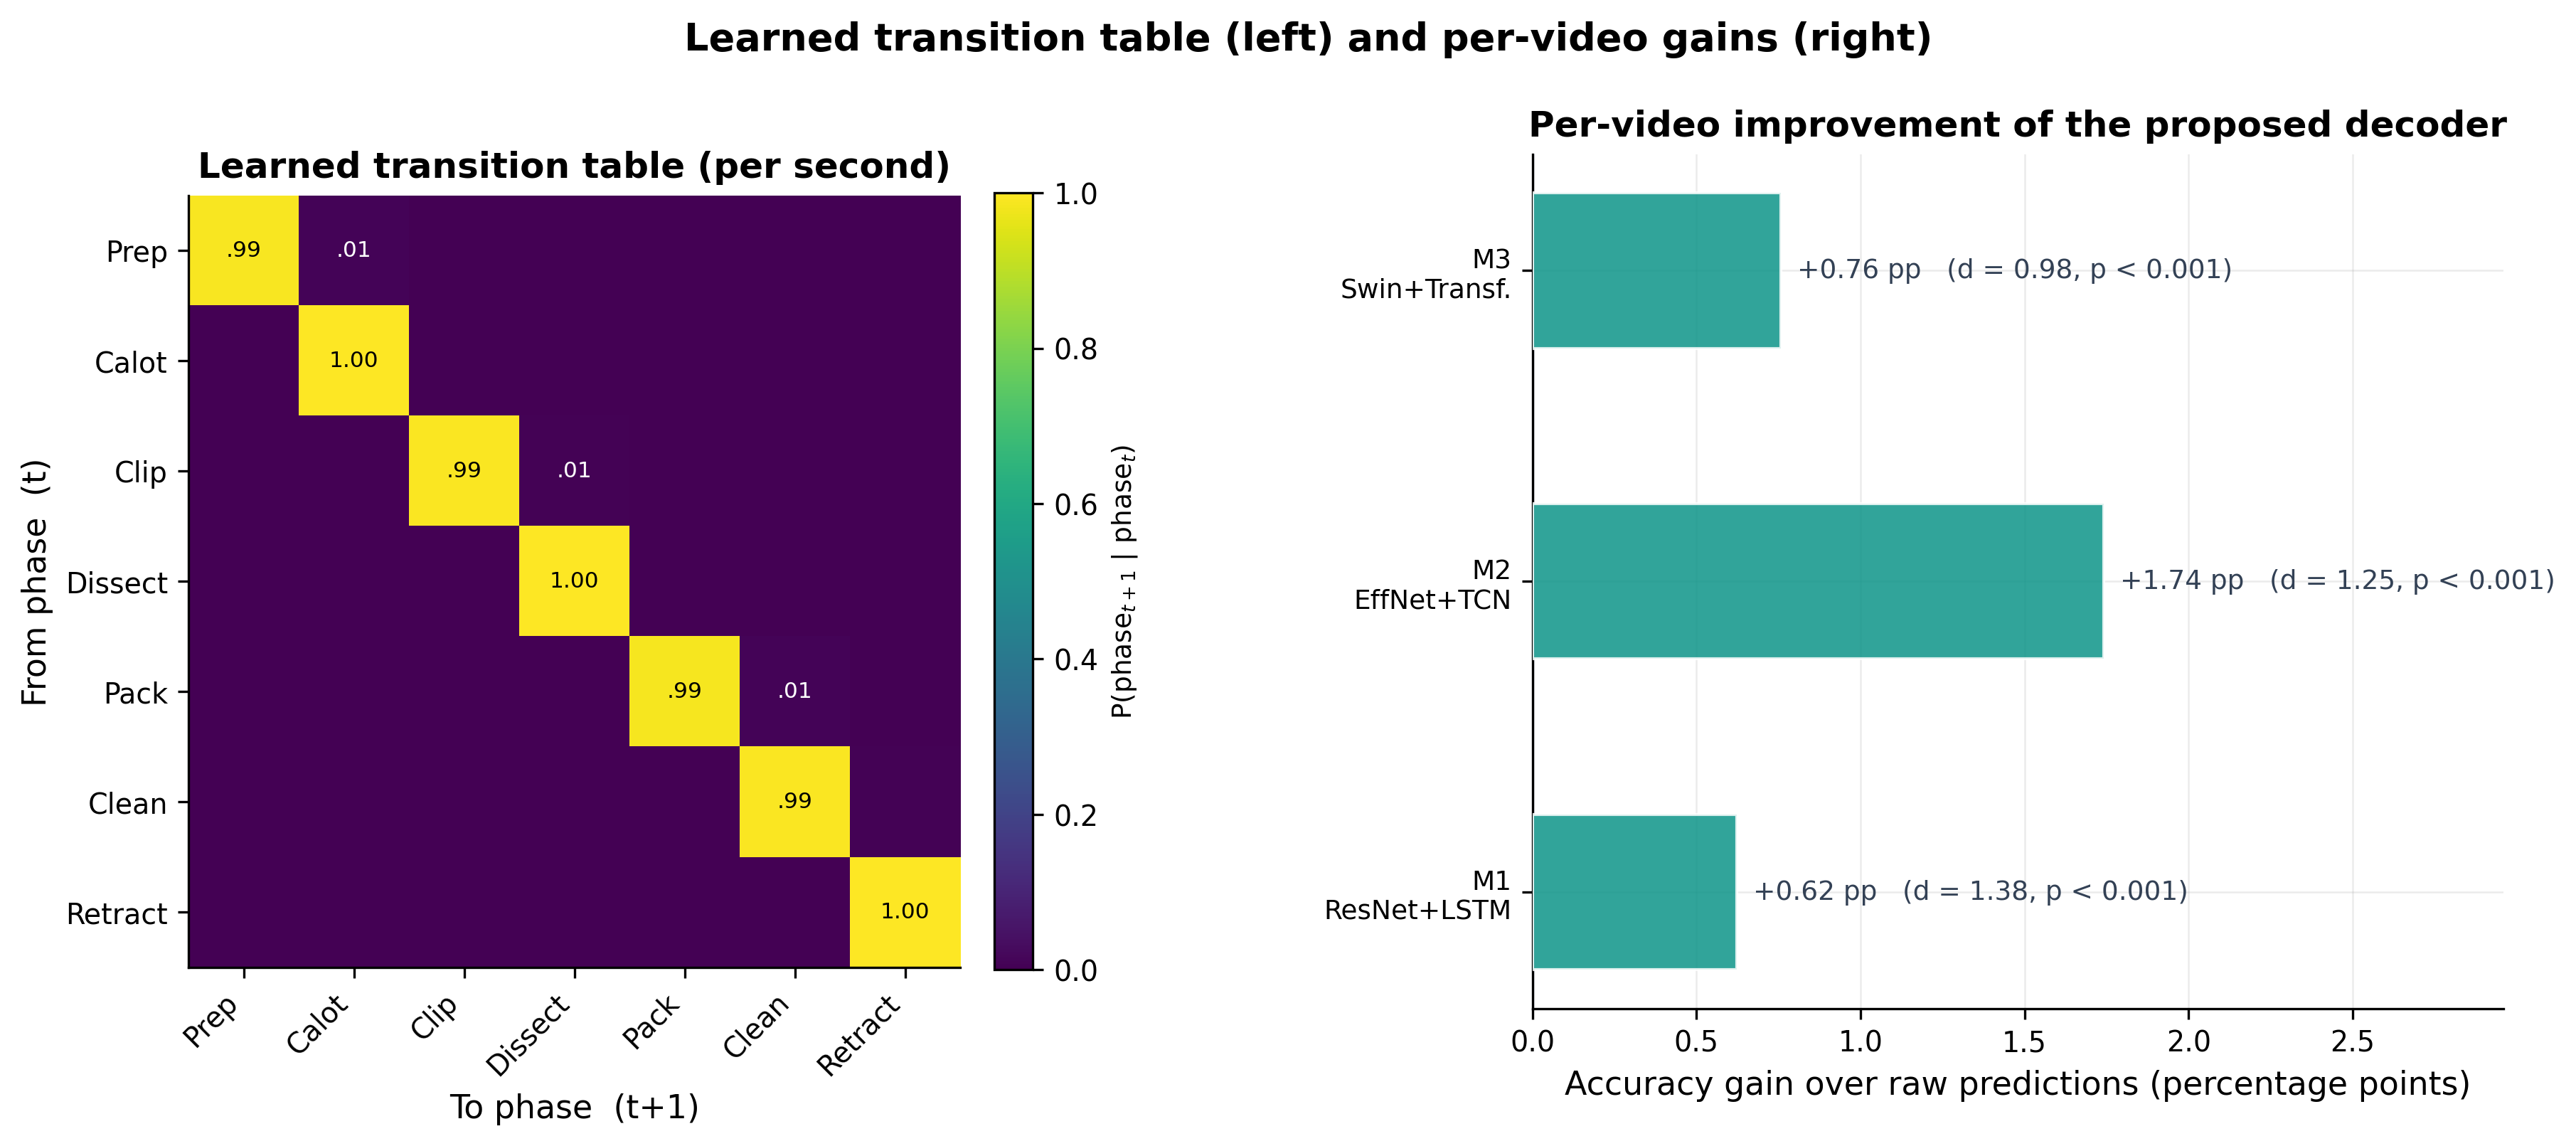
\includegraphics[width=\textwidth]{figures/transition_significance.png}
\caption{Left: the learned per-second transition table, strongly diagonal with the remaining weight on the next phase, matching the fixed phase order. Right: per-video accuracy gain of the proposed decoder over the raw predictions, with Cohen's $d$ and the Wilcoxon $p$-value.}
\label{fig:transition_significance}
\end{figure}

\subsection{Qualitative Example}

Figure~\ref{fig:timeline} shows the predicted phase timeline for one test video. The raw predictions flip back and forth, especially early on; the proposed decoder removes most of these flips and follows the ground truth much more closely.

\begin{figure}[H]
\centering
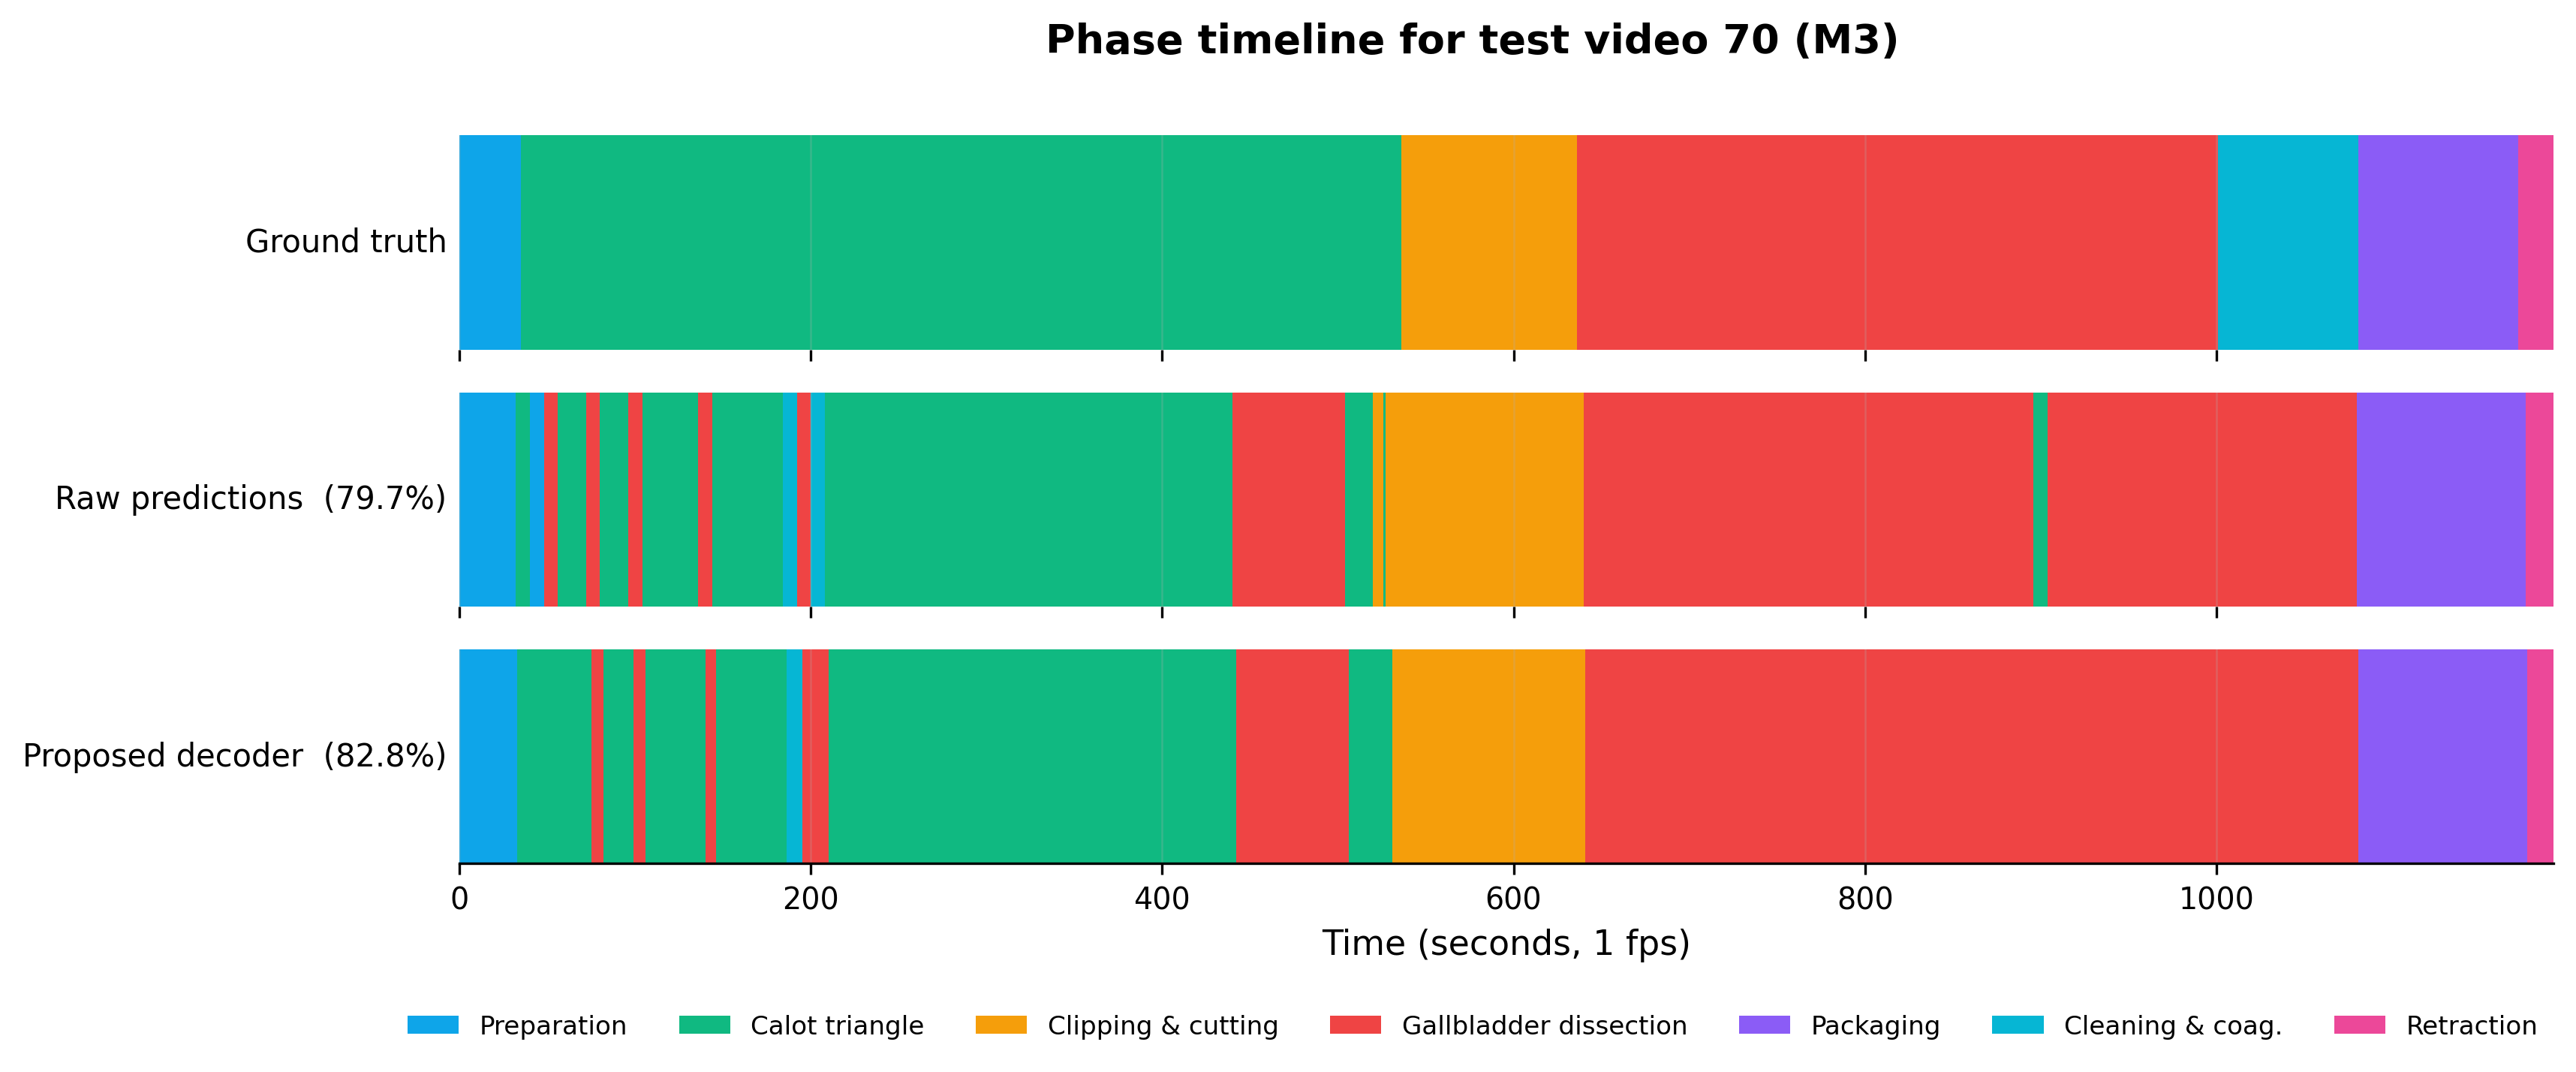
\includegraphics[width=\textwidth]{figures/timeline.png}
\caption{Phase timeline for one test video (M3). The raw predictions (middle) flip often; the proposed decoder (bottom) is much smoother and stays close to the ground truth (top).}
\label{fig:timeline}
\end{figure}

\section{Errors Near Phase Changes versus Inside Phases}
\label{sec:boundary}

On Cholec80, label disagreement is concentrated at the phase changes, where even human annotators differ on the exact moment of transition. To see where each decoder helps, the test frames are split into those \textbf{near a phase change} (within $\pm5$~s of a true transition) and those \textbf{inside a phase} (everywhere else). Table~\ref{tab:boundary} reports the split for M3, and Figure~\ref{fig:boundary} shows it.

\begin{table}[H]
\centering
\caption{Accuracy near phase changes versus inside phases, for M3. The offline decoder $\dagger$ uses future frames. Best \emph{real-time} values in \textbf{bold}.}
\label{tab:boundary}
\begin{tabular}{lcc}
\toprule
\textbf{Decoder} & \textbf{Near change} & \textbf{Inside phase} \\
\midrule
Raw predictions          & 60.7\% & 86.1\% \\
Median-15 filter         & 61.1\% & 86.3\% \\
\textbf{Proposed decoder} & \textbf{63.2\%} & 86.8\% \\
\midrule
Offline (full video) $\dagger$ & 62.8\% & 91.0\% \\
\bottomrule
\end{tabular}
\end{table}

\begin{figure}[H]
\centering
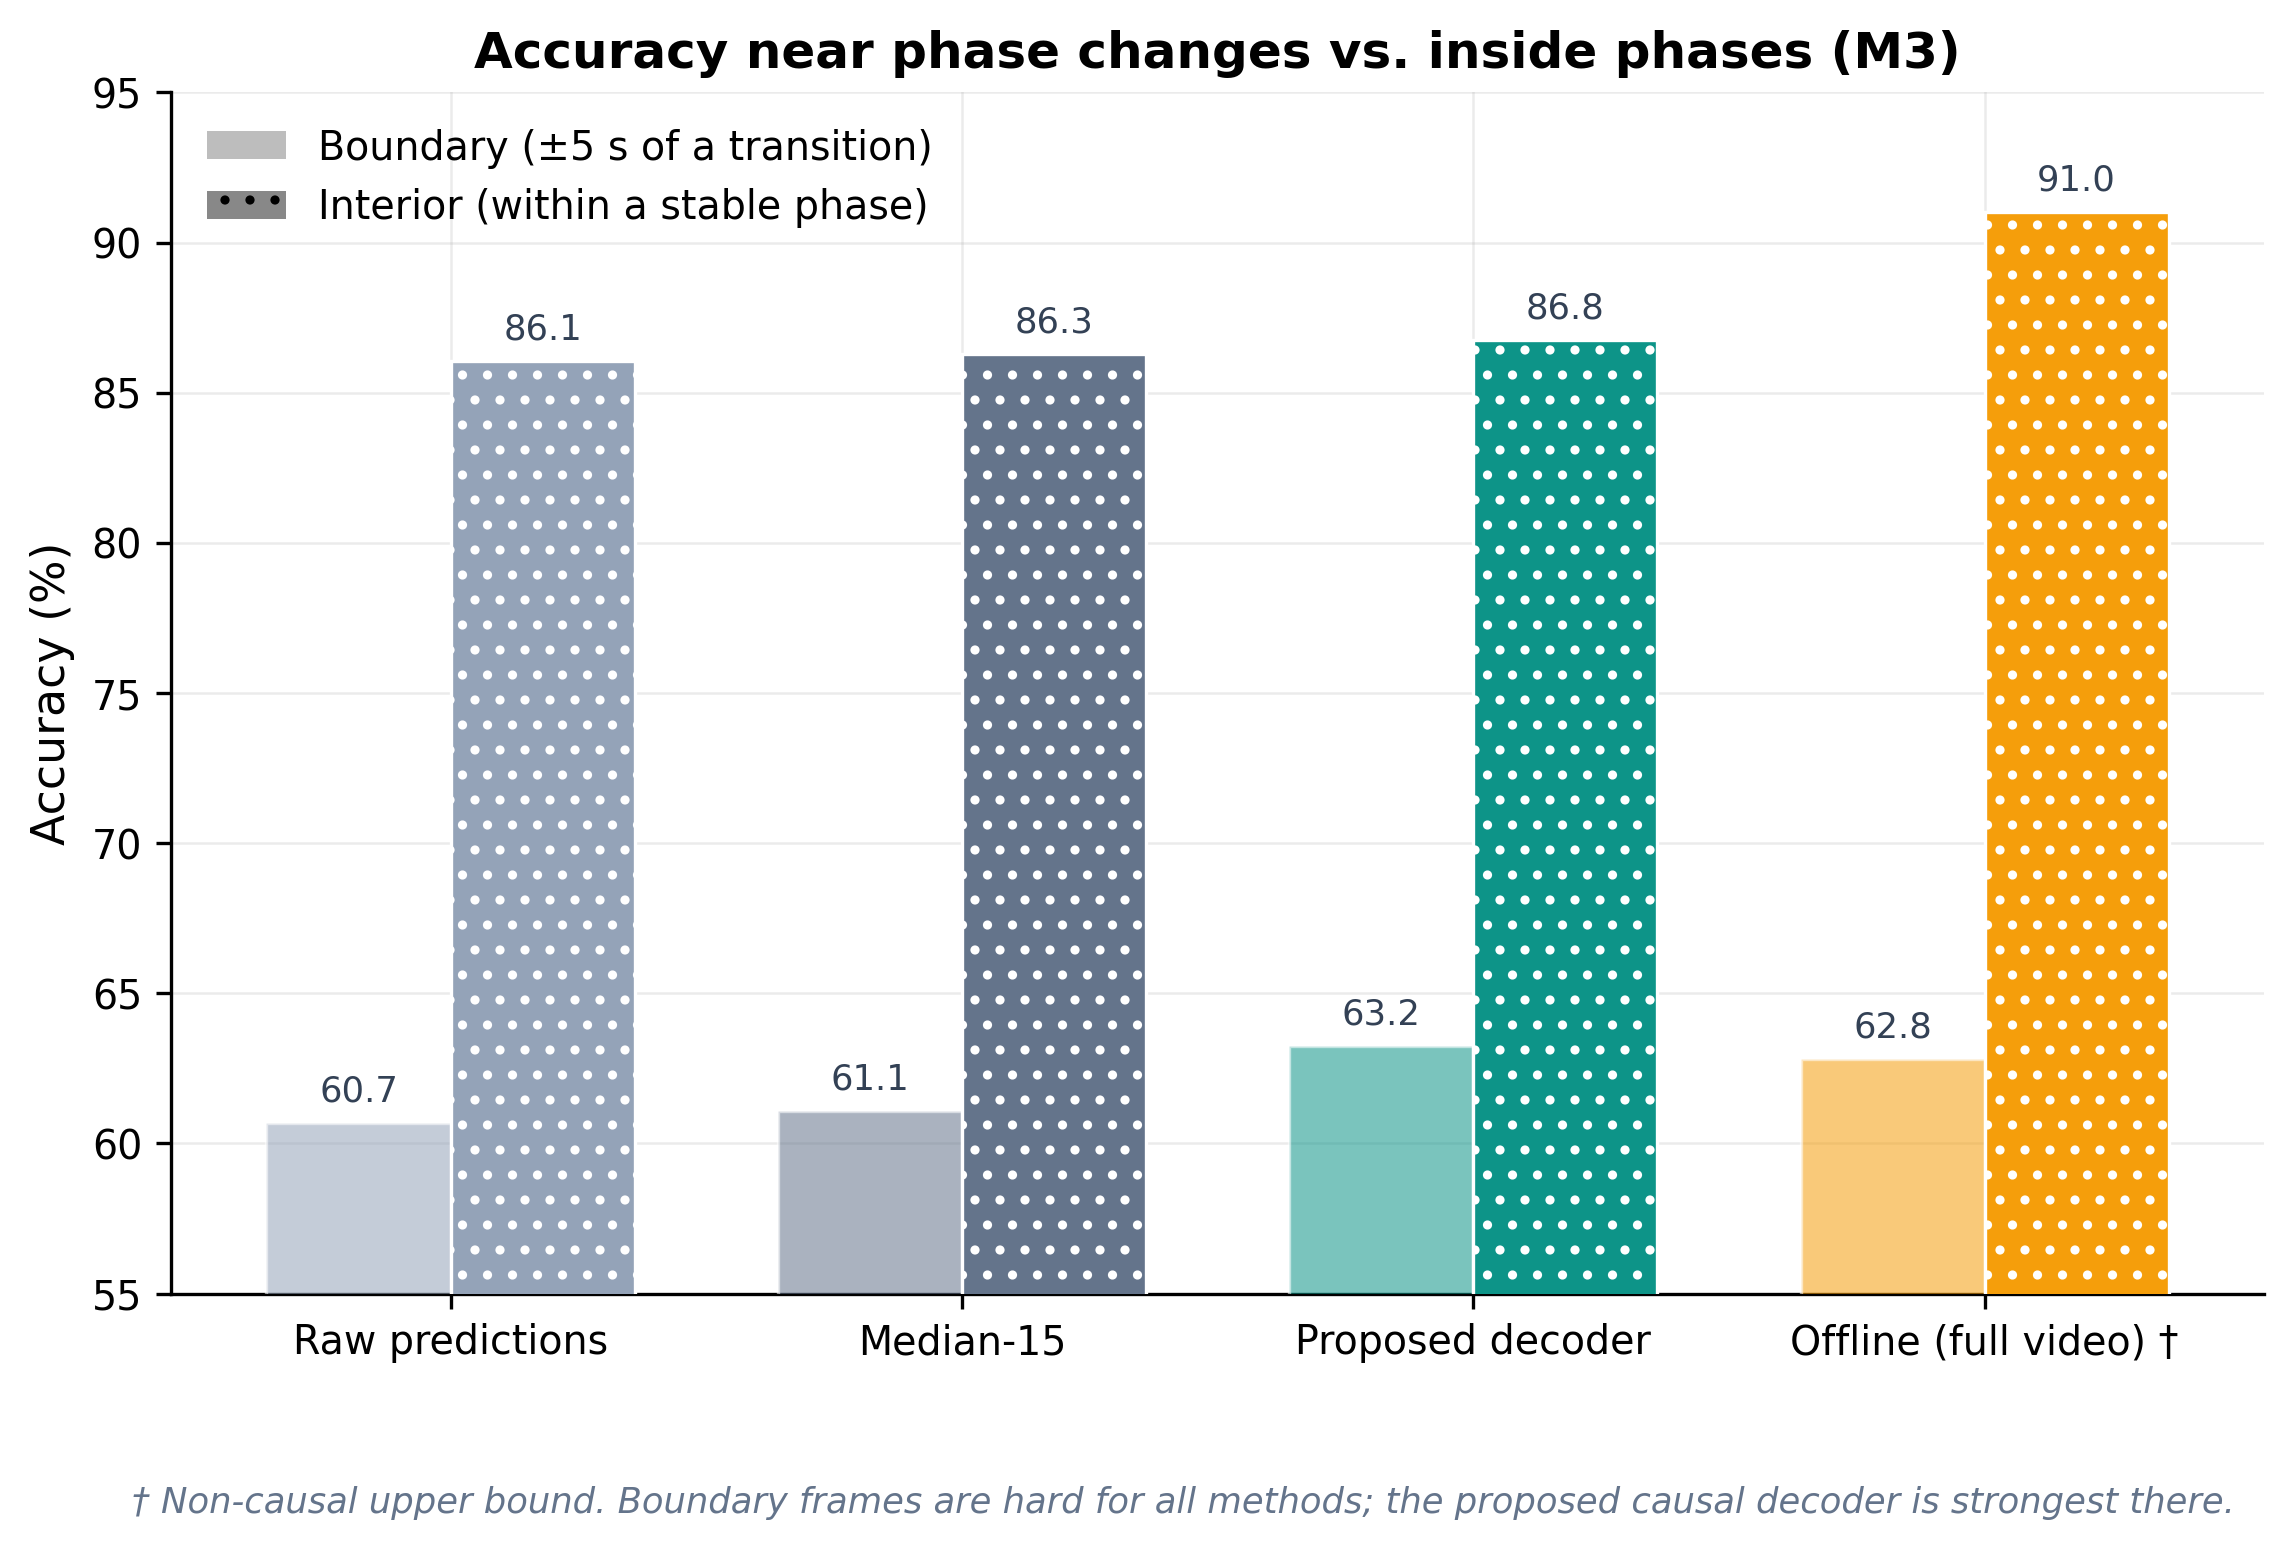
\includegraphics[width=\figwidth]{figures/boundary.png}
\caption{Accuracy near phase changes versus inside phases, for M3. Frames near a change (solid bars) are hard for every method; the proposed decoder is best there, even slightly above the offline upper bound. Inside phases (hatched bars) is where the offline decoder's advantage comes from.}
\label{fig:boundary}
\end{figure}

Two points stand out. First, the proposed decoder is the \textbf{best near phase changes} (63.2\%), even above the offline upper bound (62.8\%): the offline decoder's hard rule that phases cannot go backwards sometimes delays a transition, while the soft learned table follows the labelled timing more flexibly. Second, the whole 4.2-point gap between the offline decoder and the best real-time decoder is \emph{inside} the phases ($86.8 \to 91.0$), not at the changes. The offline decoder's advantage is fixing brief mistakes inside long stable phases by looking at future frames---something a real-time decoder cannot do. To our knowledge this split has not been measured before on Cholec80, and it points to a clear next step: letting the decoder look a few seconds ahead would close most of the gap while still being usable in near-real time.
